\documentclass[18pt, xcolor=table]{beamer}
\usepackage{xcolor}
\usepackage{templates/beamerthemekit}
\usepackage[export]{adjustbox}
\usepackage{tikz}
\usepackage{url}
\usepackage{amsmath}
\usepackage[table]{xcolor}
\usepackage{tabularx}
\usepackage{marvosym} % \MVRIGHTarrow
\usepackage{stmaryrd} % \shortrightarrow
\usepackage{textcomp} % \textrightarrow
\usepackage{svg}
\usepackage{tabularx}

\title[Research Project]{Towards Bringing Together Numerical Methods for Partial Differential Equation and Deep Neural Networks}
\subtitle{Project presentation, Supervisor - Markus Hoffmann}
\author{Stanislav Arnaudov}
\institute{Chair for Computer Architecture and Parallel Processing}
\date{4. Juni, 2020}
\selectlanguage{english}

\newcommand{\semitransp}[2][35]{\color{fg!#1}#2 \color{fg}}

\begin{document}

\begin{frame}
 \titlepage
\end{frame}

\section{Introduction}


\begin{frame}[t]
  \frametitle{Introduction}
  \textbf{Basic idea:} Apply machine learning and image processing in computational fluid dynamics context
\end{frame}

\begin{frame}[t]
  \frametitle{Introduction}
  \textbf{Basic idea:} Apply machine learning and image processing in computational fluid dynamics (CFD) context
  \begin{columns}[t]
    \begin{column}{0.5\textwidth}
      \begin{itemize}
      \item Machine learning through deep neural networks
      \item DNNs for image generation
      \end{itemize}
    \end{column}
    \begin{column}{0.5\textwidth}
    \end{column}
  \end{columns}
\end{frame}

\begin{frame}[t]
  \frametitle{Introduction}
  \textbf{Basic idea:} Apply machine learning and image processing in computational fluid dynamics (CFD) context
  \begin{columns}[t]
    \begin{column}{0.5\textwidth}
      \begin{itemize}
      \item Machine learning through deep neural networks
      \item DNNs for image generation
      \end{itemize}
    \end{column}
    \begin{column}{0.5\textwidth}
      \begin{itemize}
      \item Simulation of fluids through mathematical models
      \item Differential equations
      \item Specialized solvers for the equations
      \end{itemize}
    \end{column}
  \end{columns}
\end{frame}

\begin{frame}
  \frametitle{Project}
  \begin{itemize}
  \item \Large{\textbf{What} we aimed to do?}
  \item \Large{\textbf{Why} is our research being done?}
  \item \Large{\textbf{How} were our goals achieved?}
  \end{itemize}
\end{frame}


\section{What}

\begin{frame}[t]
  \frametitle{What}
  \begin{itemize}
  \item Predict the flow around an object in a channel.
  \end{itemize}
\end{frame}

\begin{frame}[t]
  \frametitle{What}
  \begin{itemize}
  \item Predict the flow around an object in a channel.
  \end{itemize}

  \begin{figure}[htb]
    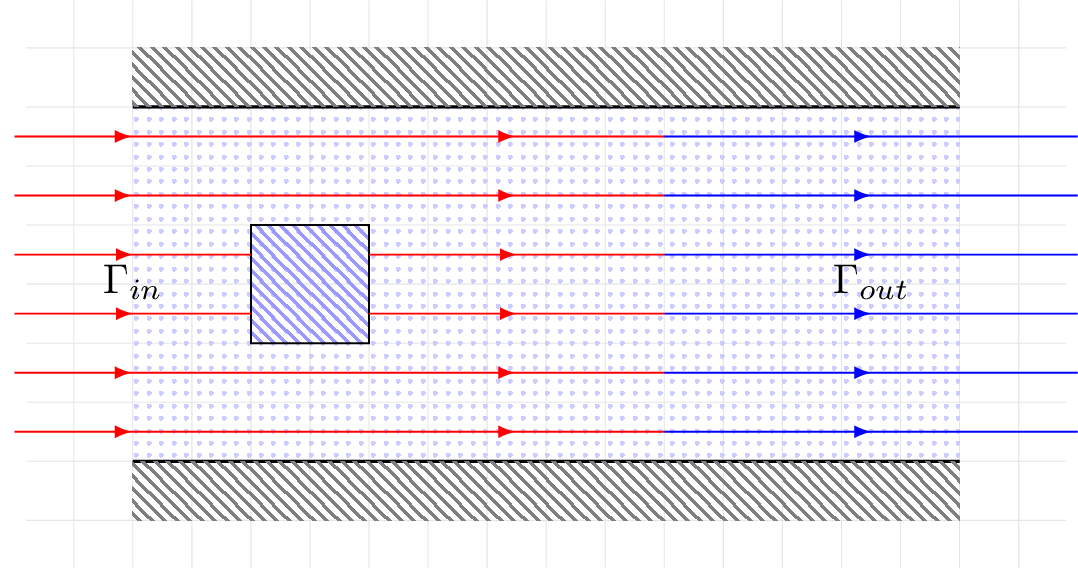
\includegraphics[scale=0.24]{images/channel/flow_2}
    \caption{Simulation Setup}
  \end{figure}

\end{frame}

\begin{frame}[t]
  \frametitle{What}
  \begin{itemize}
  \item Predict the flow around an object in a channel.
  \end{itemize}

  \begin{figure}[htb]
    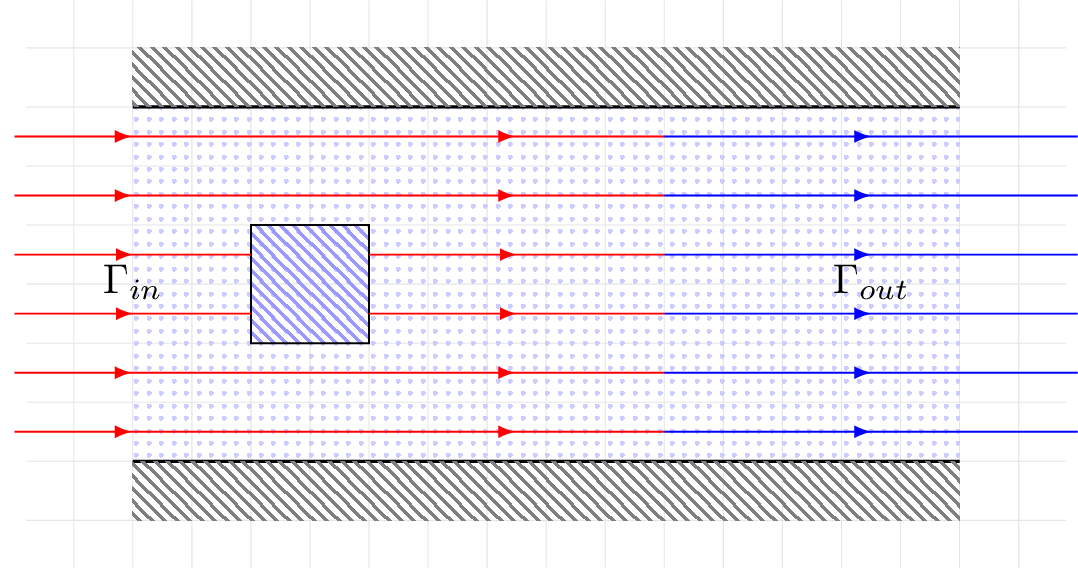
\includegraphics[scale=0.14]{images/channel/flow_2}
  \end{figure}

  \vspace{-1cm}

  \begin{columns}[t]
    \begin{column}{0.5\textwidth}
      \begin{center}
        \Large{Parameters}\\
        \small{for the whole simulation}
      \end{center}
      \begin{itemize}
      \item Inflow speed of the fluid
      \item Viscosity and density of the fluid
      \end{itemize}

    \end{column}
    \begin{column}{0.5\textwidth}
      \begin{center}
        \Large{Solutions}\\
        \small{for each timestep}
      \end{center}

      \begin{itemize}
      \item Velocity field (x\&y directions)
      \item Pressure field
      \end{itemize}

    \end{column}
  \end{columns}

\end{frame}


\begin{frame}[t]
  \frametitle{What}
  \begin{itemize}
  \item Predict the flow around an object in a channel.
  \end{itemize}
  
  \begin{figure}[htb]
    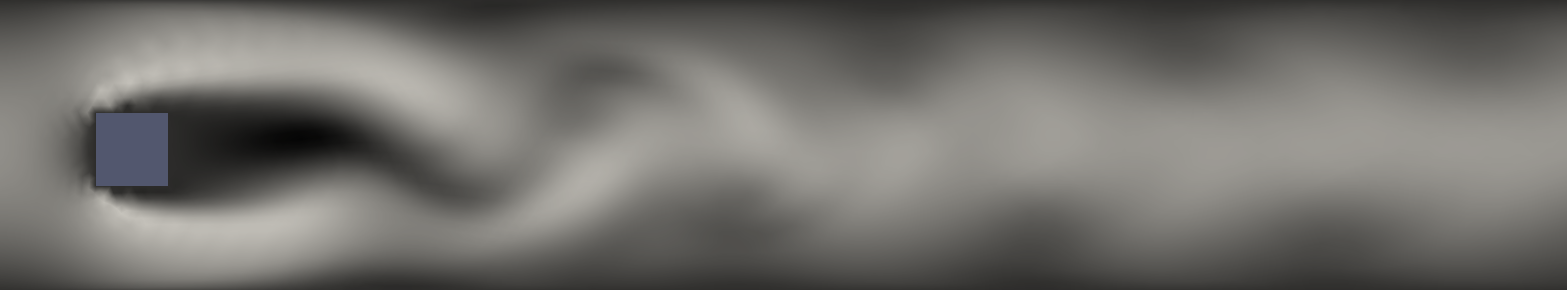
\includegraphics[scale=0.19]{images/true/flow_x}
    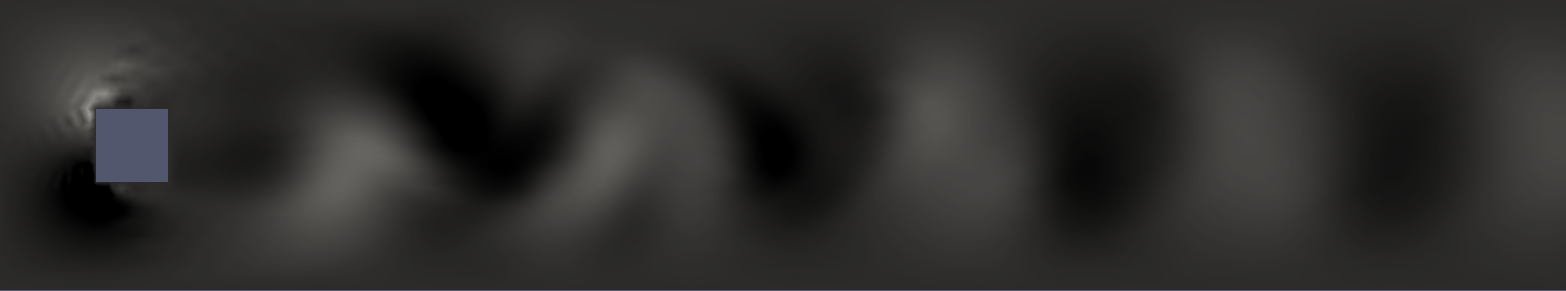
\includegraphics[scale=0.19]{images/true/flow_y}
    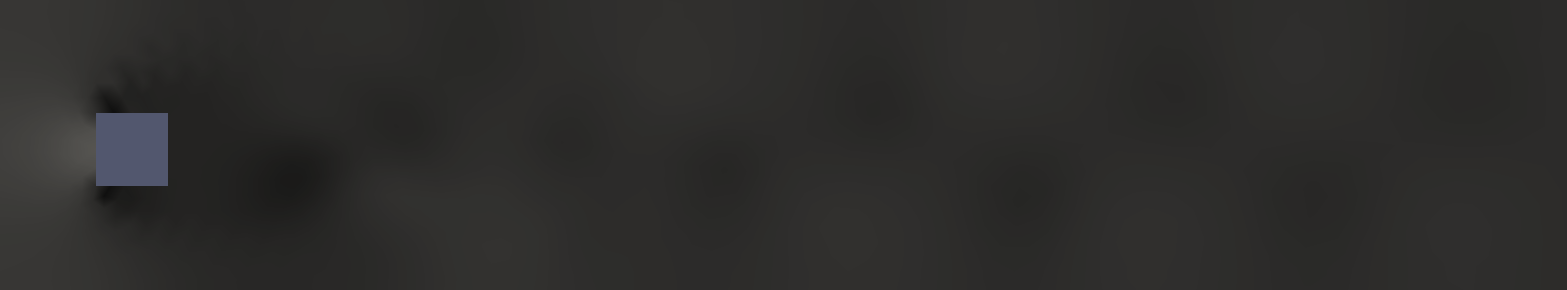
\includegraphics[scale=0.19]{images/true/flow_p}
  \end{figure}
\end{frame}

  
\begin{frame}[t]
  \frametitle{What}
  \begin{itemize}
  \item Predict the flow around an object in a channel.
  \item Network Principle
  \end{itemize}
\end{frame}


\begin{frame}[t]
  \frametitle{What}

  \begin{itemize}
  \item Predict the flow around an object in a channel.
  \item Network Principle
  \end{itemize}
  \begin{figure}[htb]
    \includegraphics[scale=0.22]{images/models/net}
  \end{figure}
\end{frame}

\section{Why}

\begin{frame}[t]
  \frametitle{Why}
\end{frame}

\begin{frame}
  \frametitle{Why}
  \begin{columns}[t]
    \begin{column}{0.5\textwidth}
      \vspace{-0.5cm}
      \begin{center}
        \begin{figure}[htb]
          \includegraphics[scale=0.2]{images/final/pipeline}
        \end{figure}
      \end{center}
    \end{column}
    \begin{column}{0.5\textwidth}
      \begin{itemize}
      \item Lots of parameters to tweak
      \item Complicated workflow
      \item Computationally expensive
      \end{itemize}
    \end{column}
  \end{columns}
\end{frame}

\begin{frame}
  \frametitle{Why}
  \begin{columns}[t]
    \begin{column}{0.5\textwidth}
      \vspace{-0.5cm}
      \begin{center}
        \begin{figure}[htb]
          \includegraphics[scale=0.2]{images/final/net}
        \end{figure}
      \end{center}
    \end{column}
    \begin{column}{0.5\textwidth}
      \begin{itemize}
      \item Everything is learned during training
      \item DNNs are well established in image processing tasks
      \item Faster image generation
      \end{itemize}
    \end{column}
  \end{columns}
\end{frame}

\section{How}

\begin{frame}[t]
  \frametitle{How}
\end{frame}

\begin{frame}[t]
  \frametitle{How}
  \begin{itemize}
  \item Not a single holistic model
  \begin{itemize}
    \item Constant model
    \item Inflow speed model
    \item Viscosity-density model
    \end{itemize}
  \end{itemize}
\end{frame}

\begin{frame}[t]
  \frametitle{How}
  \begin{itemize}
  \item Not a single holistic model
  \item Model variations
    \begin{itemize}
    \item Usage of the pressure field
    \item No usage of the pressure field
    \end{itemize}
  \end{itemize}
\end{frame}

\section{Data Generation}

\begin{frame}[t]
  \frametitle{Data Generation}
\end{frame}

\begin{frame}[t]
  \frametitle{Data Generation}
  \begin{itemize}
  \item Real simulation data gathering
    \begin{itemize}
    \item Define large amount of simulations
    \item Solving --- HiFlow3\footnotemark as numerical solver
      \footnotetext{Ayachit, Utkarsh, ``The ParaView Guide: A Parallel Visualization Application, Kitware'' , 2015, ISBN 978-1930934306}
    \item Rendering --- ParaView\footnotemark as visualization toolkit
        \footnotetext{Gawlok, S., Gerstner, P., Haupt, S., Heuveline, V., Kratzke, J., Lösel, P., Mang, K., Schmidtobreick, M., Schoch, N., Schween, N., Schwegler, J., Song, C. and Wlotzka, M., ``HiFlow3 – Technical Report on Release 2.0''}
    \end{itemize}
  \end{itemize}
\end{frame}


\begin{frame}[t]
  \frametitle{Data Generation}
  \begin{itemize}
  \item Real simulation data gathering
  \item Separate data sets for each model
    \begin{itemize}
    \item Single simulation for the constant model
    \item Multiple simulations for the other models
    \end{itemize}
  \end{itemize}
\end{frame}

\begin{frame}[t]
  \frametitle{Data Generation}
  \begin{itemize}
  \item Real simulation data gathering
  \item Separate data sets for each model
  \item Parameters for the simulations
    \begin{itemize}
    \item Not chosen at random
    \item \textit{Reynolds number} in [90, 450]
    \item Non-trivial simulations
    \end{itemize}
  \end{itemize}
\end{frame}

\begin{frame}[t]
  \frametitle{Data Generation}
  \begin{itemize}
  \item Real simulation data gathering
  \item Separate data sets for each model
  \item Parameters for the simulations
  \end{itemize}
  \begin{center}
    \begin{figure}[htb]
      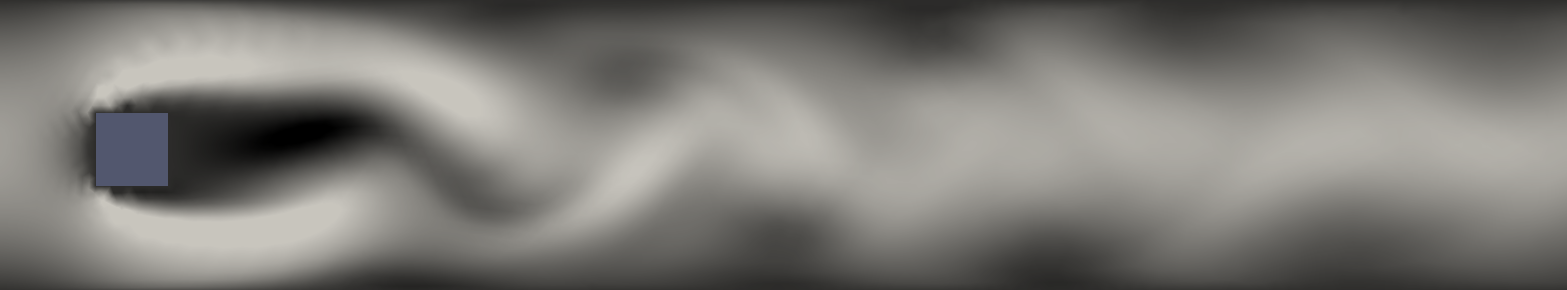
\includegraphics[scale=0.2]{images/flows/flow_x}
      \caption{X velocity}
      \vspace{-0.2cm}
    \end{figure}

    \begin{figure}[htb]
      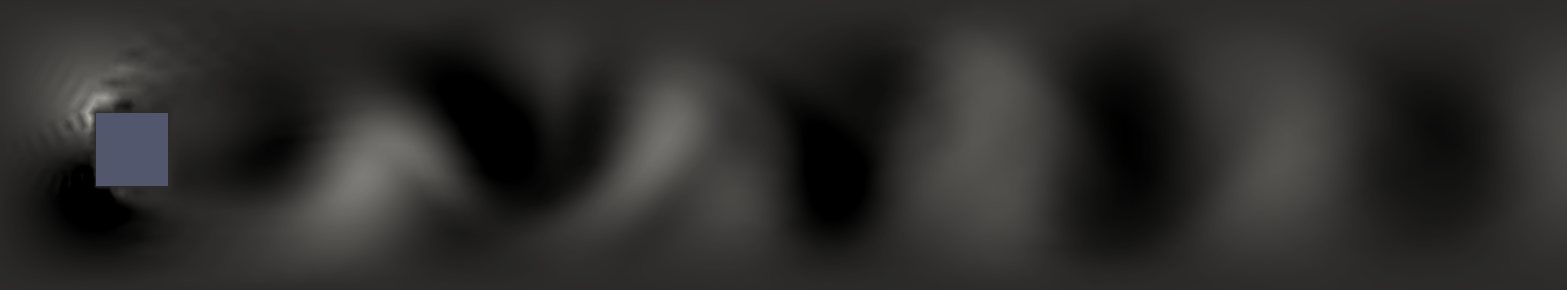
\includegraphics[scale=0.2]{images/flows/flow_y}
      \vspace{-0.2cm}
      \caption{Y velocity}
    \end{figure}
  \end{center}
\end{frame}

\begin{frame}[t]
  \frametitle{Data Generation}

  \begin{itemize}
  \item Real simulation data gathering
  \item Separate data sets for each model
  \item Parameters for the simulations
  \item Test train splits
    \begin{itemize}
    \item 80\slash20 split for all data sets
    \item No common Reynolds numbers between the simulations in the train- and test-sets
    \end{itemize}
  \end{itemize}
\end{frame}


\section{Models}

\begin{frame}[t]
  \frametitle{Networks Architectures}
\end{frame}

\begin{frame}[t]
  \frametitle{Networks Architectures}
  \begin{itemize}
  \item Real numbers handling
  \end{itemize}
\end{frame}

\begin{frame}[t]
  \frametitle{Networks Architectures}
  \begin{itemize}
  \item Real numbers handling
  \end{itemize}
  \begin{center}
    \begin{figure}[htb]
      \includegraphics[scale=0.23]{images/models/num_answer}
    \end{figure}
  \end{center}
\end{frame}

\begin{frame}[t]
  \frametitle{Networks Architectures}
  \begin{itemize}
  \item Real numbers handling
  \item Approach based on Pix2Pix\footnotemark
    \begin{itemize}
    \item General image-to-image translation framework
    \item Impressive results in recent years
    \end{itemize}
  \end{itemize}

  \begin{center}
    \begin{figure}[htb]
      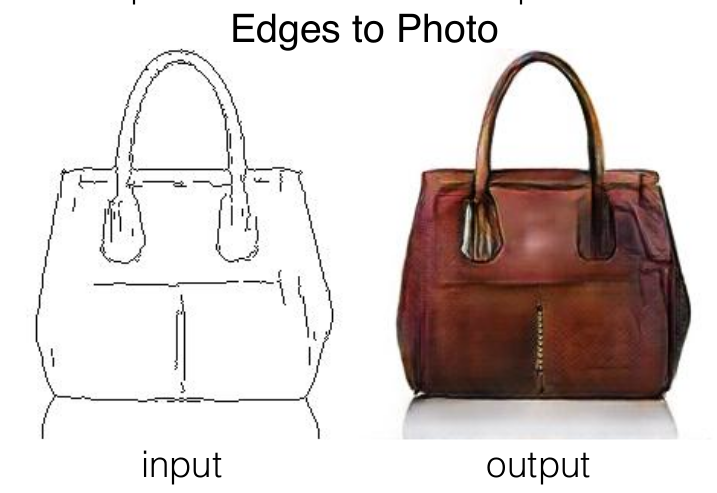
\includegraphics[scale=0.23]{images/pix2pix_example}
      \vspace{-0.5cm}
      \caption{Example image from the pix2pix paper}
    \end{figure}
  \end{center}

  \footnotetext{Ting-Chun Wang, Ming-Yu Liu, Jun-Yan Zhu, Andrew Tao, Jan Kautz, and Bryan Catanzaro. ``High-resolution image synthesis and semantic manipulation with conditional gans.''}
\end{frame}

\begin{frame}[t]
  \frametitle{Networks Architectures}
  \begin{itemize}
  \item Real numbers handling
  \item Approach based on Pix2Pix
  \item Conditional GAN (cGAN)
  \end{itemize}
  \begin{center}
    \begin{figure}[htb]
      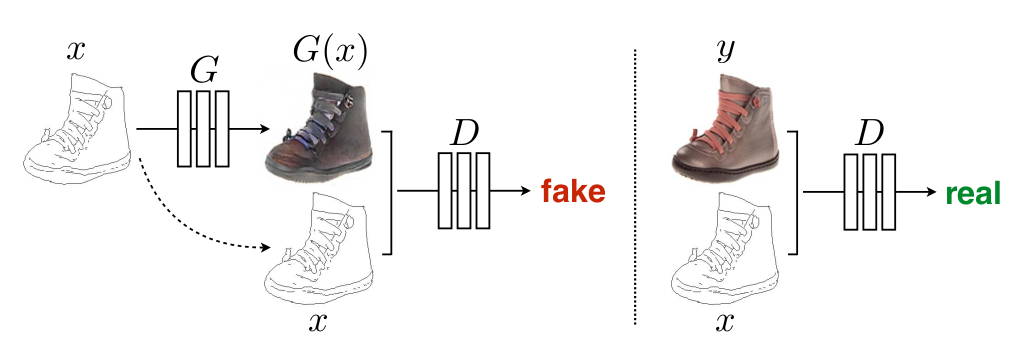
\includegraphics[scale=0.33]{images/pix2pix_cgan}
      \caption{Training a cGAN}
    \end{figure}
  \end{center}

\end{frame}


\begin{frame}[t]
  \frametitle{Networks Architectures}
  \begin{itemize}
  \item Real numbers handling
  \item Approach based on Pix2Pix
  \item Conditional GAN (cGAN)
  \item Generator Architecture
    \begin{itemize}
    \item UNet
    \end{itemize}
  \end{itemize}

  \begin{center}
    \begin{figure}[htb]
      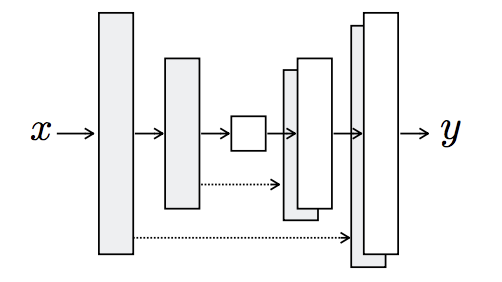
\includegraphics[scale=0.33]{images/nets/unet}
      \caption{The UNet architecture}
    \end{figure}
  \end{center}

\end{frame}


\begin{frame}[t]
  \frametitle{Networks Architectures}
  \begin{itemize}
  \item Real numbers handling
  \item Approach based on Pix2Pix
  \item Conditional GAN (cGAN)
  \item Generator Architecture
  \item Discriminator Architecture
    \begin{itemize}
    \item PatchGAN
    \end{itemize}
  \end{itemize}

\end{frame}

\section{Evaluation}

\begin{frame}[t]
  \frametitle{Evaluation}
\end{frame}

\begin{frame}[t]
  \frametitle{Evaluation}
  \begin{itemize}
  \item Evaluation Strategies
  \end{itemize}
  \vspace{-0.7cm}
  \begin{columns}[t]
    \begin{column}{0.5\textwidth}
      \begin{center}
        {\large \underline{Individual Images}}
        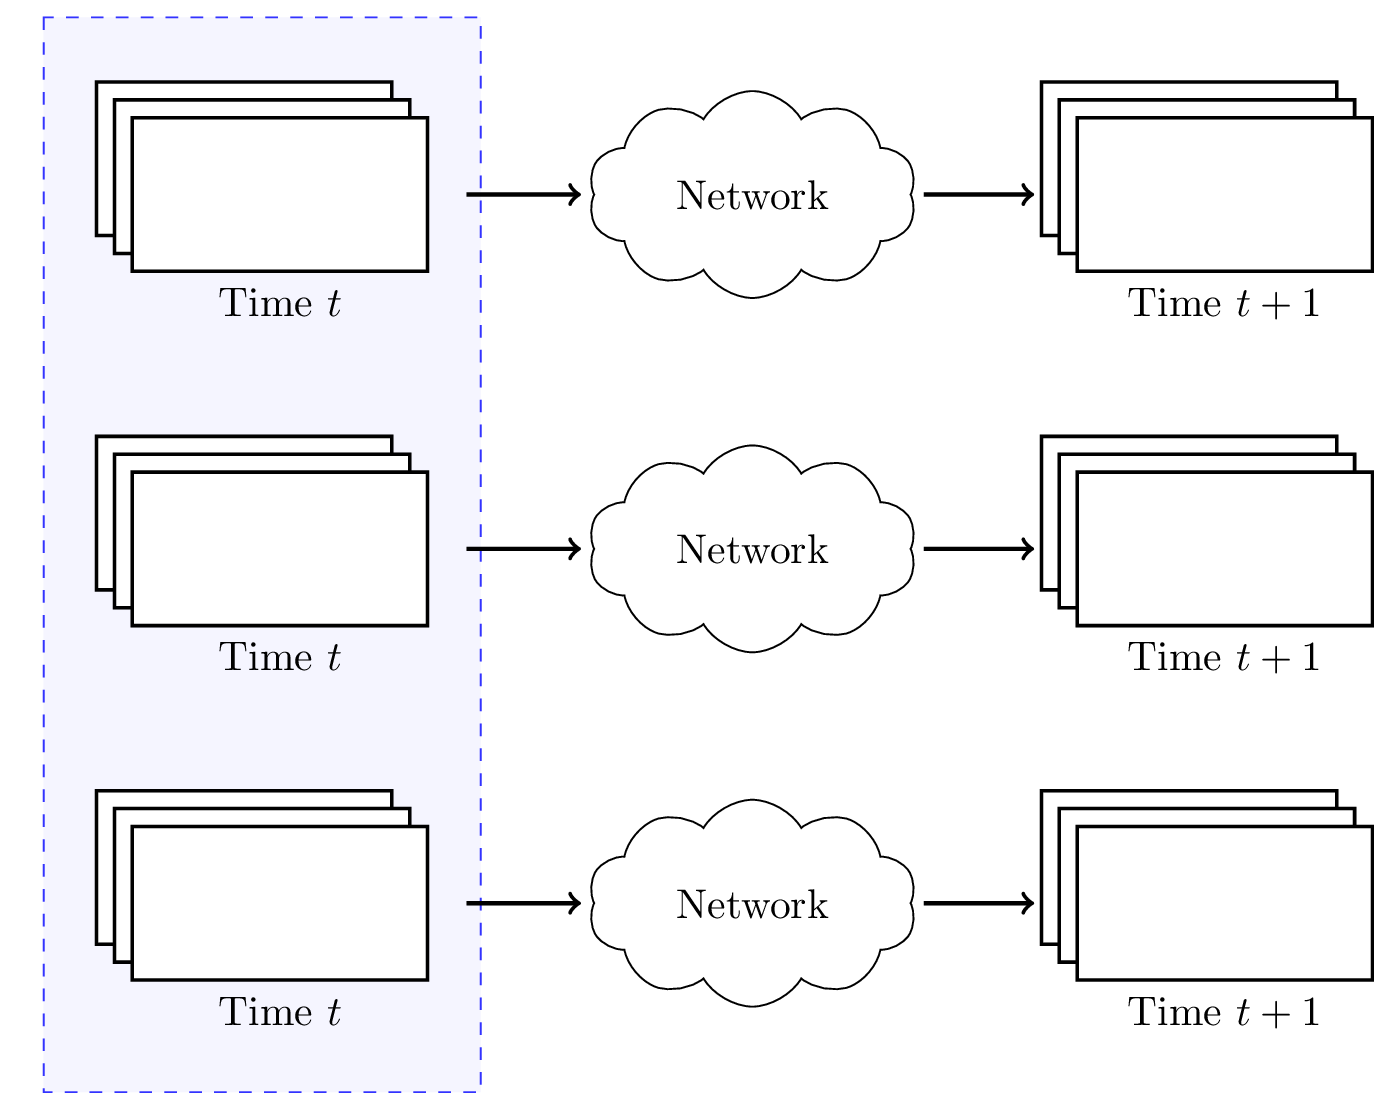
\includegraphics[scale=0.12]{images/simple_eval}
      \end{center}
    \end{column}
    \begin{column}{0.5\textwidth}
      \begin{center}
        {\large \underline{Recursive Application}}
        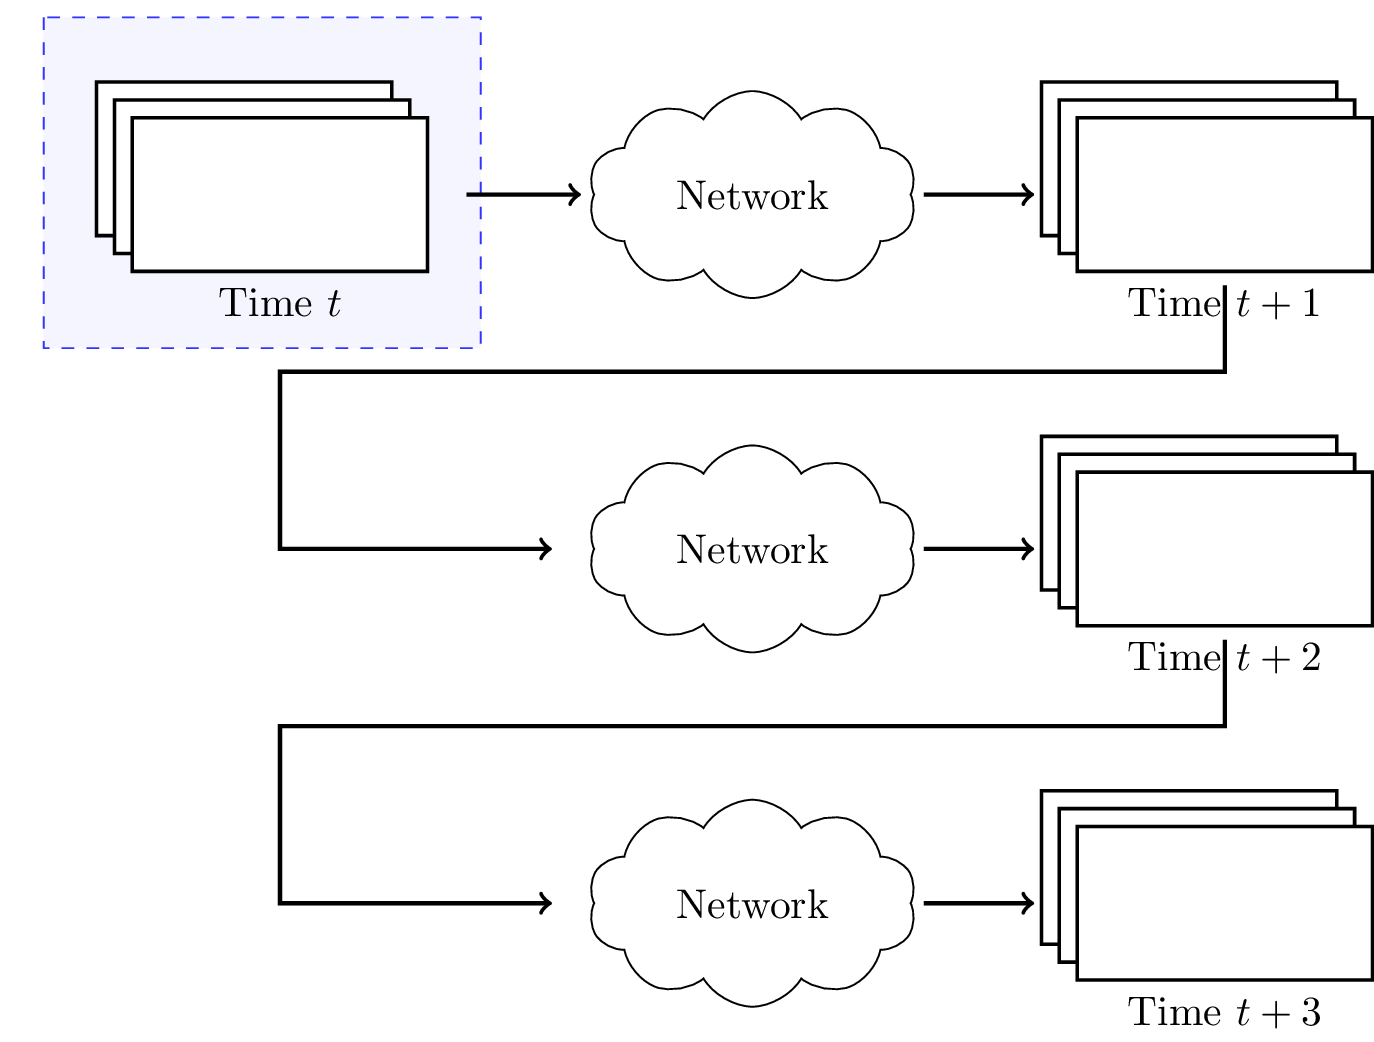
\includegraphics[scale=0.12]{images/rec_eval}
      \end{center}
    \end{column}
  \end{columns}
\end{frame}

\begin{frame}[t]
  \frametitle{Evaluation}
  \begin{itemize}
  \item Evaluation Strategies
  \item Results Views
    \begin{itemize}
    \item Numerical point of view
    \item Perceptual\slash Visual point of view
    \end{itemize}
  \end{itemize}
\end{frame}

\begin{frame}[t]
  \frametitle{Evaluation}
  \large{Numerical View}
  \begin{itemize}
  \item Average difference
  \item Maximal difference
  \end{itemize}
\end{frame}

\begin{frame}[t]
  \frametitle{Evaluation}
  \large{Numerical View}
  \vspace{1.5cm}
  \begin{center}
    \begin{table}
      \rowcolors{2}{blue!15}{white}
      \begin{tabular}{|c|c|c|}
        \hline
        \rowcolor{blue!50}
        \textbf{Model}    & \textbf{Max diff.} & \textbf{Average diff.} \\
        \hline
        Constant          & 14.56\% & 0.60\%  \\
        Inflow speed      & 32.16\% & 0.55\%  \\
        Viscosity-density & 57.00\% & 13.85\% \\
        \hline
      \end{tabular}
      \caption{All of the results are from models using the pressure field}
    \end{table}
  \end{center}

\end{frame}

\begin{frame}[t]
  \frametitle{Evaluation}
  \large{Numerical View}
  \vspace{1.5cm}
  \begin{center}
    \begin{table}
      \rowcolors{2}{blue!15}{white}
      \begin{tabular}{|c|c|c|}
        \hline
        \rowcolor{blue!50}
        \textbf{Model}                       & \textbf{Max diff.} & \textbf{Average diff.} \\
        \hline
        \color{gray!!140}{Constant}          & \color{gray!!140}{14.56\%} & \color{gray!!140}{0.60\%}  \\
        \rowcolor{gray!50}
        \color{red}{Inflow speed}            & \color{red}{32.16\%} & \color{red}{0.55\%}  \\
        \color{gray!!140}{Viscosity-density} & \color{gray!!140}{57.00\%} & \color{gray!!140}{13.85\%} \\
        \hline
      \end{tabular}
      \caption{All of the results are from models using the pressure field}
    \end{table}
  \end{center}
\end{frame}

\begin{frame}[t]
  \frametitle{Evaluation}
  \large{Numerical View}
  \vspace{1.5cm}
  \begin{figure}[htb]
    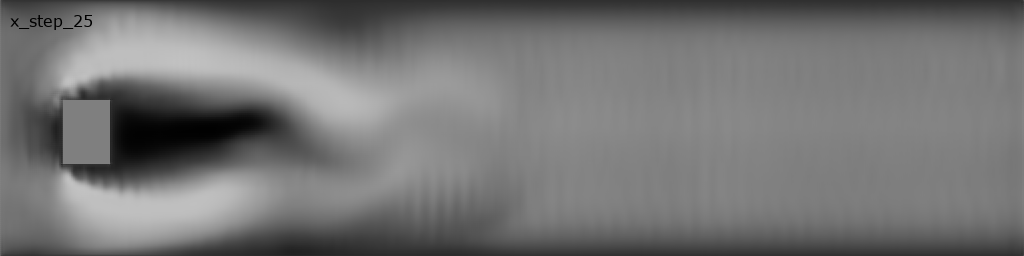
\includegraphics[scale=0.29]{images/bad_pattern}
    \caption{Visible pattern in a generated image}
  \end{figure}
\end{frame}

\begin{frame}[t]
  \frametitle{Evaluation}
  \large{Perceptual view}
  \begin{itemize}
  \item Correlation
  \item PSNR (Peak Signal to Noise Ration)
  \end{itemize}
\end{frame}

\begin{frame}[t]
  \frametitle{Evaluation}
  \large{Perceptual view}
  \begin{itemize}
  \item \textbf{Correlation}
  \item PSNR (Peak Signal to Noise Ration)
  \end{itemize}
\end{frame}

\begin{frame}[t]
  \frametitle{Evaluation}
  \large{Perceptual view}
  \begin{itemize}
  \item \textbf{Correlation}
  \item PSNR (Peak Signal to Noise Ration)
  \end{itemize}
  \begin{center}
    \begin{figure}[htb]
      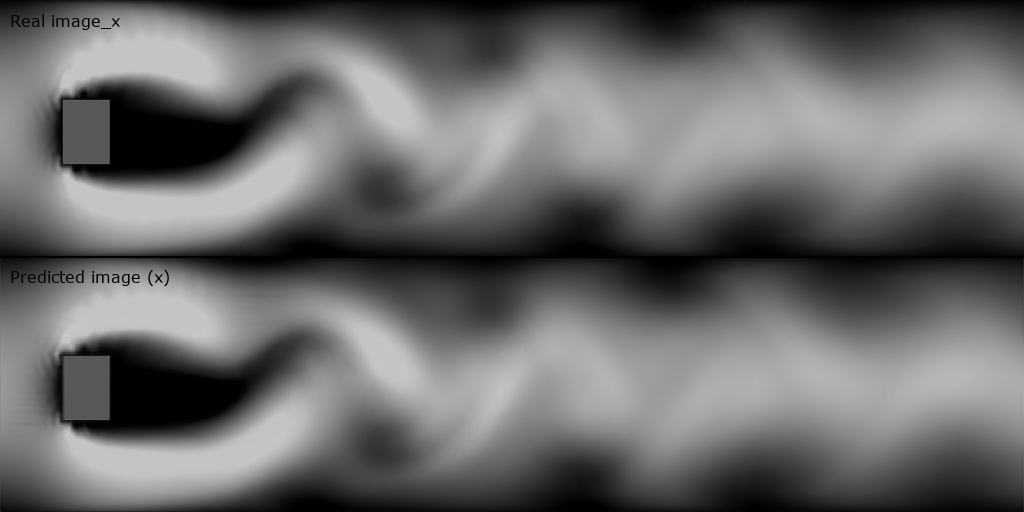
\includegraphics[scale=0.23]{images/res/prediction}
    \end{figure}
  \end{center}
\end{frame}

\begin{frame}[t]
  \frametitle{Evaluation}
  \large{Perceptual view}
  \begin{itemize}
  \item Correlation
  \item \textbf{PSNR (Peak Signal to Noise Ration)}
  \end{itemize}
\end{frame}

\begin{frame}[t]
  \frametitle{Evaluation}
  \large{Perceptual view:} \textit{PSNR} --- higher is better
  \vspace{-0.5cm}
  \begin{columns}[t]
    \begin{column}{0.5\textwidth}
      \begin{center}
        \begin{figure}[htb]
          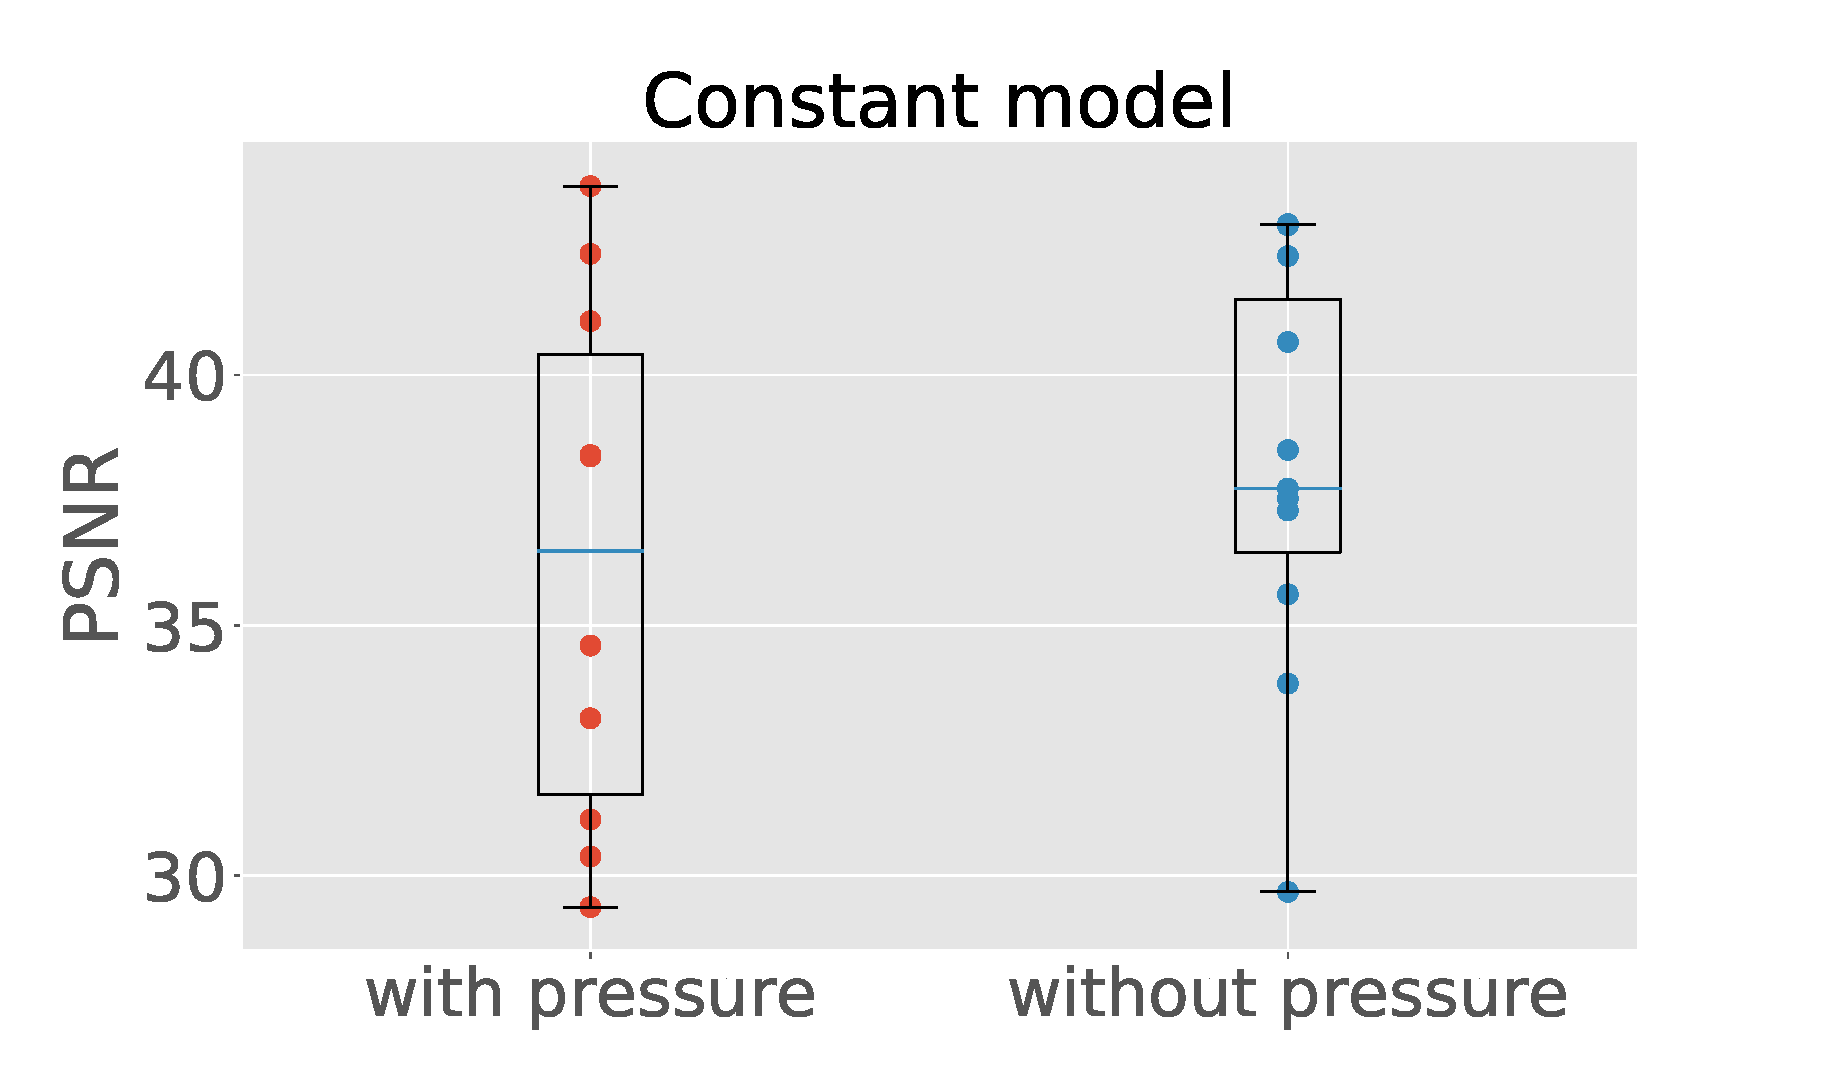
\includegraphics[scale=0.17]{images/final/single_const_psnr}
        \end{figure}
      \end{center}
    \end{column}
    \begin{column}{0.5\textwidth}
      \begin{center}
        \begin{figure}[htb]
          \includegraphics[scale=0.17]{images/final/single_speed_psnr}
        \end{figure}
      \end{center}
    \end{column}
  \end{columns}
  \begin{center}
    \begin{figure}[htb]
      \includegraphics[scale=0.17]{images/final/single_fluid_psnr}
    \end{figure}
  \end{center}
\end{frame}

\begin{frame}[t]
  \frametitle{Evaluation}
  \begin{center}
    \begin{figure}[htb]
      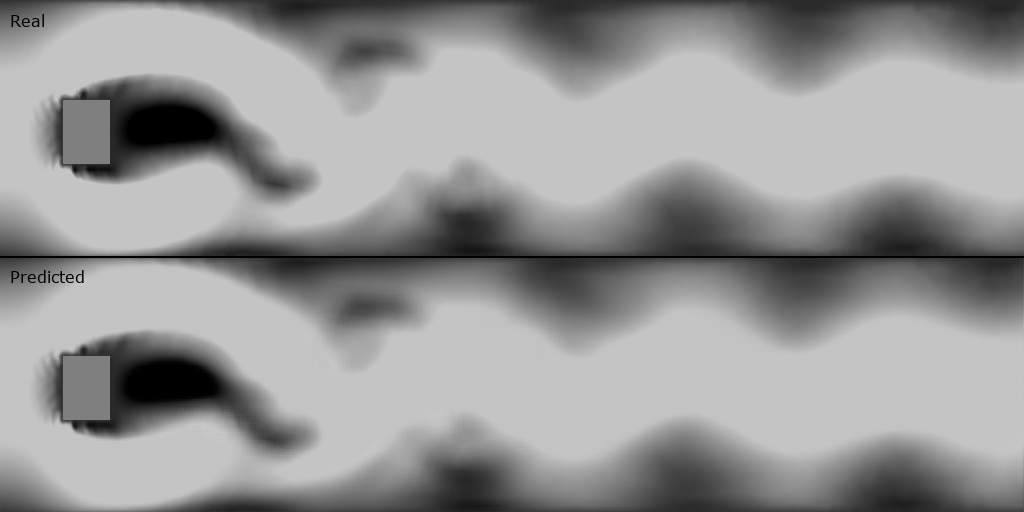
\includegraphics[scale=0.15]{images/flows/x_speed_good}
      \vspace{-0.2cm}
      \caption{Inflow speed model}
    \end{figure}
    \begin{figure}[htb]
      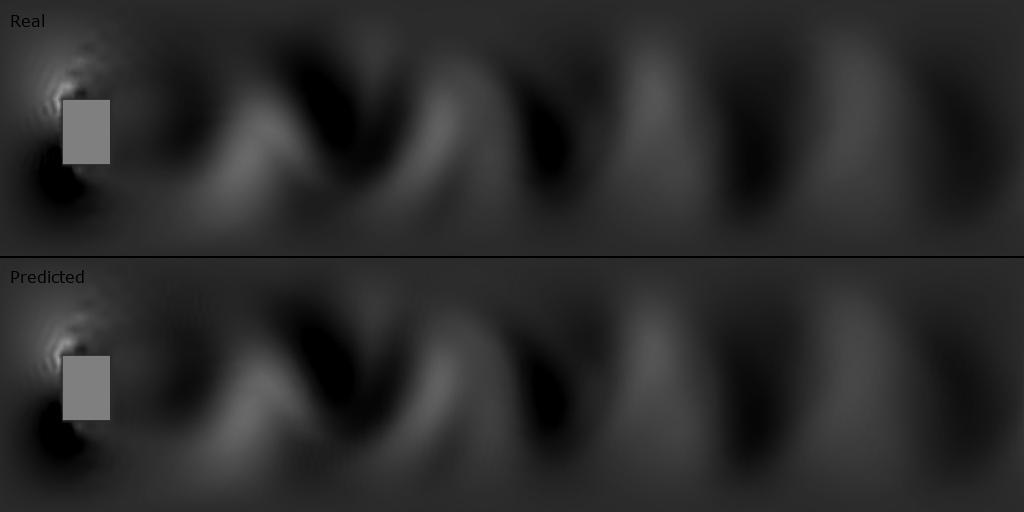
\includegraphics[scale=0.15]{images/flows/y_fluid_good}
      \vspace{-0.2cm}
      \caption{Fluid model}
    \end{figure}
  \end{center}
\end{frame}

\begin{frame}[t]
  \frametitle{Evaluation}
  \large{Perceptual view:} \textit{PSNR} --- higher is better
  \begin{center}
    \begin{figure}[htb]
      \includegraphics[scale=0.17]{images/rec_plot/inflow_39_s0}
      \includegraphics[scale=0.17]{images/rec_plot/inflow_39_s120}
      \caption{Inflow speed model recursive results}
    \end{figure}
  \end{center}
\end{frame}


\begin{frame}[t]
  \frametitle{Evaluation}
  \large{Perceptual view}
  \begin{center}
    \begin{figure}[htb]
    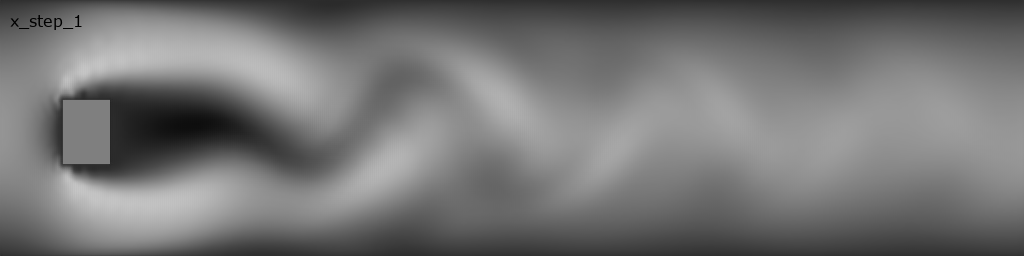
\includegraphics[scale=0.15]{images/rec_flow/x_step_1}
    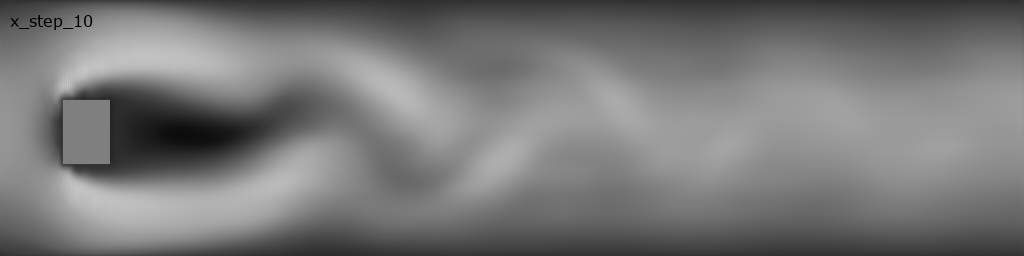
\includegraphics[scale=0.15]{images/rec_flow/x_step_10}
    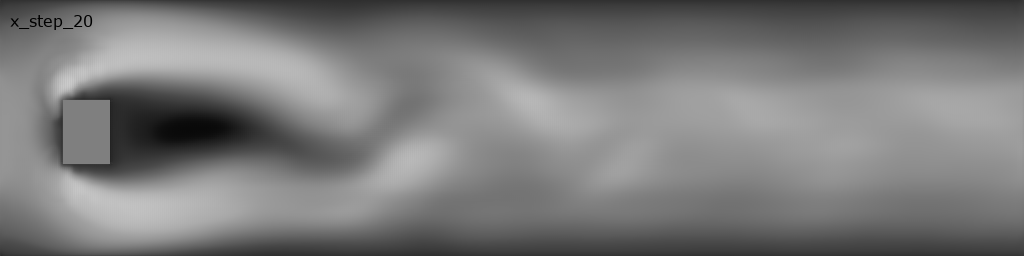
\includegraphics[scale=0.15]{images/rec_flow/x_step_20}
    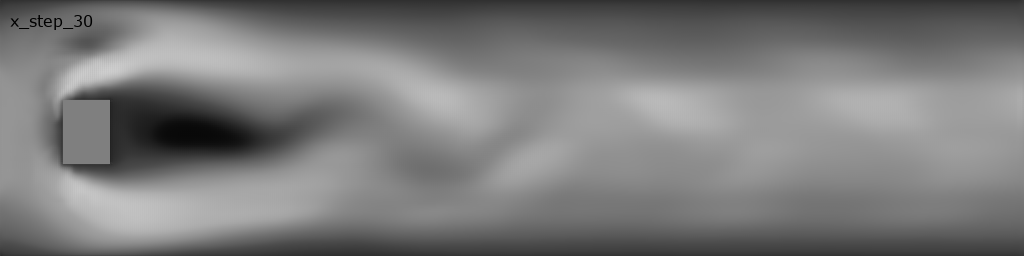
\includegraphics[scale=0.15]{images/rec_flow/x_step_30}
    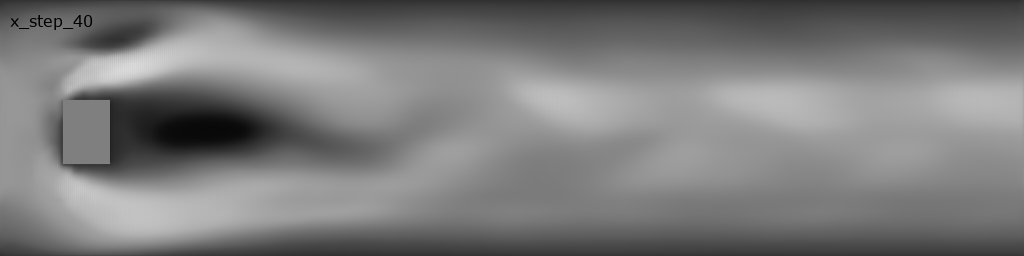
\includegraphics[scale=0.15]{images/rec_flow/x_step_40}
    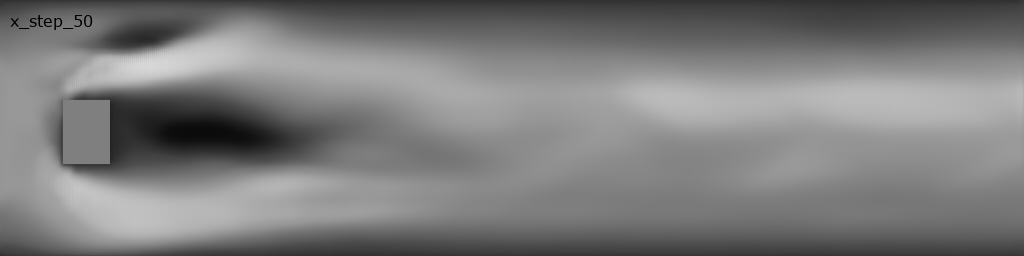
\includegraphics[scale=0.15]{images/rec_flow/x_step_50}
    \caption{Predicted simulation from the viscosity-density model}
  \end{figure}
  \end{center}
\end{frame}

\begin{frame}[t]
  \frametitle{Performance}  
\end{frame}

\begin{frame}[t]
  \frametitle{Performance}
  \vspace{1.5cm}
    \begin{center}
    \begin{table}
      \rowcolors{2}{blue!15}{white}
      \begin{tabular}{|c|c|c|c|}
        \hline
        \rowcolor{blue!50}
        \textbf{Method} & \textbf{Single core} & \textbf{Multi-Core (12)} & \textbf{GPU} \\
        \hline
        Our Networks    & $\approx 600ms$   & $\approx 100ms$  &  $4ms$ \\
        HiFlow3         & $\approx 8000ms$  & $\approx 1000ms$ & --  \\
        \hline
      \end{tabular}
      \caption{Time in milliseconds needed per simulation-step}
    \end{table}
  \end{center}
  
\end{frame}

\section{Conclusion}

\begin{frame}
  \frametitle{}
  \begin{center}
    \huge{Thank you for your attention.}
  \end{center}
\end{frame}

\begin{frame}
  \frametitle{}
  \begin{center}
    \huge{Questions?}
  \end{center}
\end{frame}

\end{document}

%%% Local Variables:
%%% mode: latex
%%% TeX-master: t
%%% End:

